\documentclass[12pt]{article}
\usepackage{fancyhdr}
\pagestyle{fancy}
\fancyhf{}
\fancyfoot[C]{\thepage}
\fancyfoot[L]{\scriptsize CC BY-NC-SA 4.0 \textbullet\ Leo Liang}
\renewcommand{\headrulewidth}{0pt}
\usepackage[margin=1in]{geometry}
\usepackage{amsmath, amssymb}
\usepackage{array, booktabs}
\usepackage{pgffor}
\usepackage{tikz}
\parindent=0pt
\parskip=1em
\newcolumntype{C}[1]{>{\centering\arraybackslash}p{#1}}
\newcommand{\wl}{\par\vspace{5mm}\noindent\rule{\linewidth}{0.4pt}\par\vspace{1mm}}
\newcommand{\wls}[1]{\foreach \i in {1,...,#1}{\wl}}
\newcommand{\gridaxes}[1]{%
  \draw[step=1,gray!25,very thin] (-#1,-#1) grid (#1,#1);%
  \draw[thick,->] (-#1-0.4,0)--(#1+0.4,0) node[right]{\scriptsize$x$};%
  \draw[thick,->] (0,-#1-0.4)--(0,#1+0.4) node[above]{\scriptsize$y$};%
  \foreach \n in {-#1,...,#1}{\ifnum\n=0\else
      \draw (\n,0.07)--(\n,-0.07) node[below]{\tiny$\n$};
      \draw (0.07,\n)--(-0.07,\n) node[left]{\tiny$\n$};\fi}%
}
% blank grid used inside the plotting problems; optional first arg = scale
\newcommand{\blankgrid}[2][0.5]{%
  \begin{tikzpicture}[scale=#1]\gridaxes{#2}\end{tikzpicture}}
% ─────────────────────────────────────────────────────────────────────────────
\begin{document}
\pagestyle{fancy}
\begin{center}
  {\Large\bfseries Homework I --- Graphing Quadratics}\\[4pt]
  Vertex Form, Completing the Square \& Putting It Together\\[4pt]
  Name: \;\underline{\hspace{4cm}}\quad Date: \; \underline{\hspace{4cm}}
\end{center}
\hrule\bigskip
\section*{Instructions}
Use a \textbf{pencil} and \textbf{show your work}. Try each problem yourself before checking anything. You are allowed to use AI for help, but always try the problem yourself first.
% ===========================================================================
\section*{Reading 0 --- Vertex Form, at a Glance}
Every quadratic can be written in \textbf{vertex form}
\[
  y = a(x-h)^2 + k .
\]
The three parameters each have one job:
\begin{itemize}
  \item $a$ controls how ``steep" the parabola is, $h$ shifts the parabola left/right, and $k$ shifts it up/down. The vertex sits at
        $(h,\,k)$, and the axis of symmetry is the vertical line $x = h$.
  \item \textbf{Be careful of the sign of $h$.} The form has a \emph{minus}: $(x-h)$. So $y=(x-3)^2$ has its vertex at
        $(3,0)$, while $y=(x+1)^2 = (x-(-1))^2$ has its vertex at $(-1,0)$.
\end{itemize}
% ===========================================================================
\newpage
\section*{Section 1 --- Graphing from Vertex Form (and backwards)}
\subsection*{Reading --- a reliable way to graph}
Given $y=a(x-h)^2+k$, graph it in four steps:
\begin{enumerate}
  \item Plot the vertex $(h,k)$.
  \item Use $a$ to decide which way it opens (up or down) and how steep it is.
\end{enumerate}
\subsection*{Going backward --- from a graph to an equation}
To read an equation off a graph: the vertex gives you $h$ and $k$ immediately. You can then look at how the height changes to find $a$. However, for not-so-obvious $a$'s, such as $a = 3/4$, this will be hard to see by eye. So a more reliable method that will always work is to pick one more
point $(x,y)$ that the curve clearly passes through, substitute it in, and solve for $a$.
\textbf{\textit{Example}}
\begin{center}
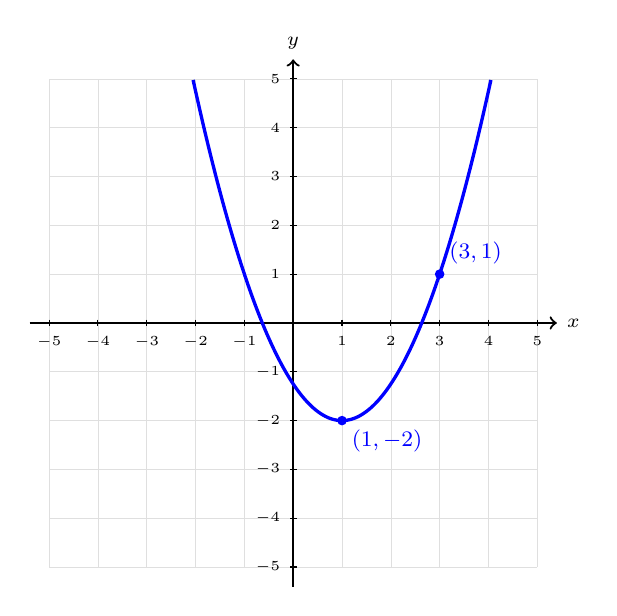
\begin{tikzpicture}[scale=0.62]
  \gridaxes{5}
  \draw[very thick,blue,domain=-2.05:4.05,samples=150] plot(\x,{(3/4)*(\x-1)^2-2});
  \fill[blue] (1,-2) circle (2.8pt) node[below right]{\footnotesize $(1,-2)$};
  \fill[blue] (3,1) circle (2.8pt) node[above right]{\footnotesize $(3,1)$};
\end{tikzpicture}
\end{center}
The parabola above has its vertex at $(1,-2)$, so $h=1$ and $k=-2$:
\[ y = a(x-1)^2 - 2 . \]
The stretch factor $a$ is not something you can read off by eye here --- it turns out to be a fraction. So use one
more point the curve clearly passes through, say $(3,1)$, and substitute it for $x$ and $y$:
\[ 1 = a(3-1)^2 - 2 \quad\Longrightarrow\quad 1 = 4a - 2 \quad\Longrightarrow\quad 4a = 3 \quad\Longrightarrow\quad a = \frac{3}{4} . \]
So the equation is $y = \tfrac{3}{4}(x-1)^2 - 2$. (Why does this method work?)
\subsection*{Problems 1--10 --- graph each quadratic}
Mark the vertex, then plot enough points to show the shape.

\medskip
\foreach \eq/\lbl in {%
  {y=(x-2)^2-3}/1, {y=(x+1)^2-4}/2, {y=-(x-1)^2+3}/3, {y=-(x+2)^2+2}/4,
  {y=2(x-1)^2-2}/5, {y=\tfrac{1}{2}(x+2)^2-3}/6, {y=-2(x-2)^2+4}/7, {y=(x-3)^2-1}/8,
  {y=-(x+3)^2+4}/9, {y=\tfrac{1}{2}(x-1)^2-2}/10}{%
  \begin{minipage}[t]{0.48\linewidth}
    \textbf{\lbl.}\quad $\displaystyle \eq$\\[2pt]
    \centering\blankgrid[0.575]{5}
  \end{minipage}\hfill
  \ifodd\lbl\else\par\bigskip\fi
}
\newpage
\subsection*{Problems 11--15 --- write the equation of each graph}
Each graph is a parabola in the form $y=a(x-h)^2+k$. Read off the vertex, use one more point (if necessary), and write the equation. 

\medskip
% R1: y=(x+1)^2-2
\begin{minipage}[t]{0.48\linewidth}
\textbf{11.}\\[2pt]
\centering
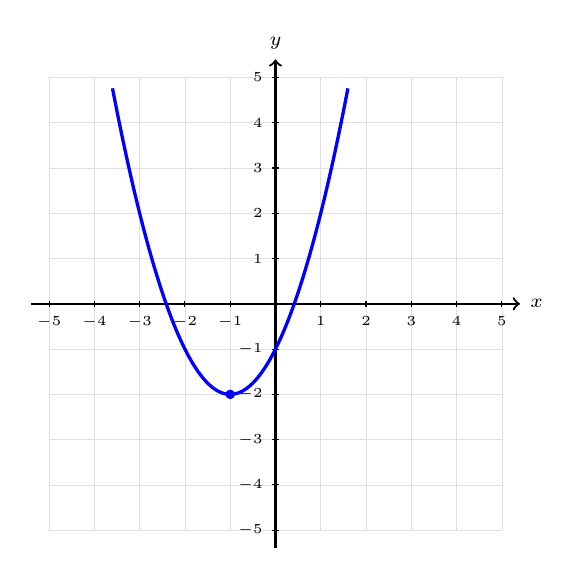
\begin{tikzpicture}[scale=0.575]
  \gridaxes{5}
  \draw[very thick,blue,domain=-3.6:1.6,samples=100] plot(\x,{(\x+1)^2-2});
  \fill[blue] (-1,-2) circle (3pt);
\end{tikzpicture}
\par\vspace{9mm}\raggedright Equation: \underline{\hspace{4.5cm}}
\end{minipage}\hfill
% R2: y=-(x-2)^2+3
\begin{minipage}[t]{0.48\linewidth}
\textbf{12.}\\[2pt]
\centering
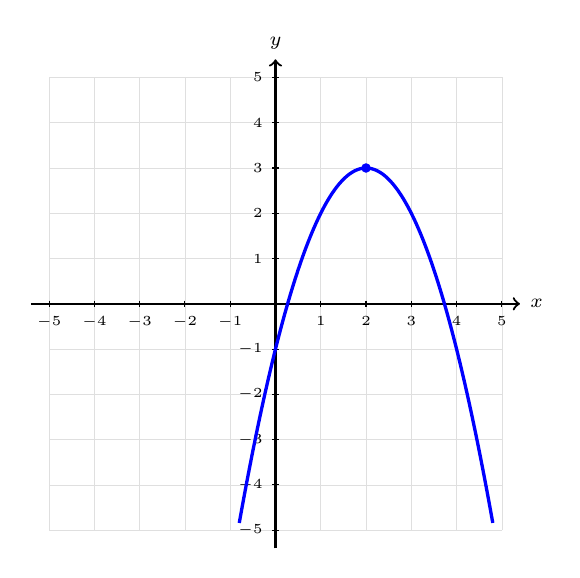
\begin{tikzpicture}[scale=0.575]
  \gridaxes{5}
  \draw[very thick,blue,domain=-0.8:4.8,samples=100] plot(\x,{-(\x-2)^2+3});
  \fill[blue] (2,3) circle (3pt);
\end{tikzpicture}
\par\vspace{9mm}\raggedright Equation: \underline{\hspace{4.5cm}}
\end{minipage}
\par\vspace{12mm}
% R3: y=2(x+2)^2-1
\begin{minipage}[t]{0.48\linewidth}
\textbf{13.}\\[2pt]
\centering
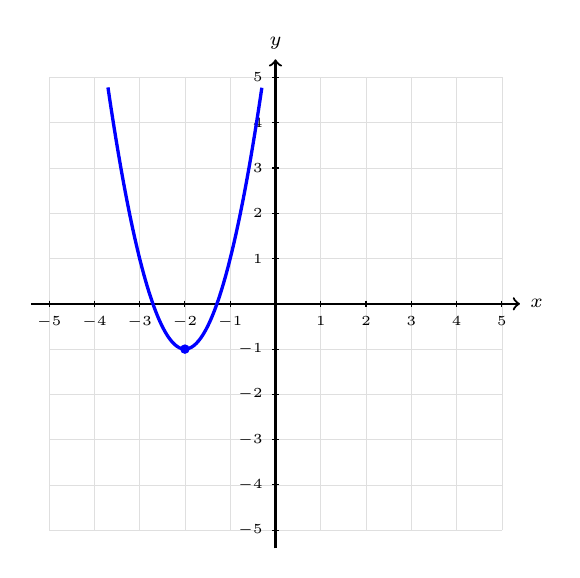
\begin{tikzpicture}[scale=0.575]
  \gridaxes{5}
  \draw[very thick,blue,domain=-3.7:-0.3,samples=100] plot(\x,{2*(\x+2)^2-1});
  \fill[blue] (-2,-1) circle (3pt);
\end{tikzpicture}
\par\vspace{9mm}\raggedright Equation: \underline{\hspace{4.5cm}}
\end{minipage}\hfill
% R4: y=(3/4)(x+2)^2-1   [a = 3/4]
\begin{minipage}[t]{0.48\linewidth}
\textbf{14.} (Notice $a$ is not so visually obvious)\\[2pt]
\centering
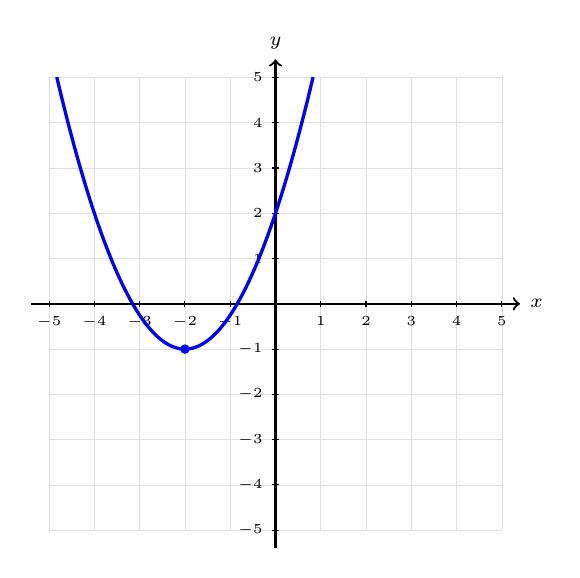
\begin{tikzpicture}[scale=0.575]
  \gridaxes{5}
  \draw[very thick,blue,domain=-4.83:0.83,samples=120] plot(\x,{(3/4)*(\x+2)^2-1});
  \fill[blue] (-2,-1) circle (3pt);
\end{tikzpicture}
\par\vspace{9mm}\raggedright Equation: \underline{\hspace{4.5cm}}
\end{minipage}

% R5: y=-(3/4)(x-1)^2+2   [a = -3/4]
\begin{minipage}[t]{0.48\linewidth}
\textbf{15.}\\[2pt]
\centering
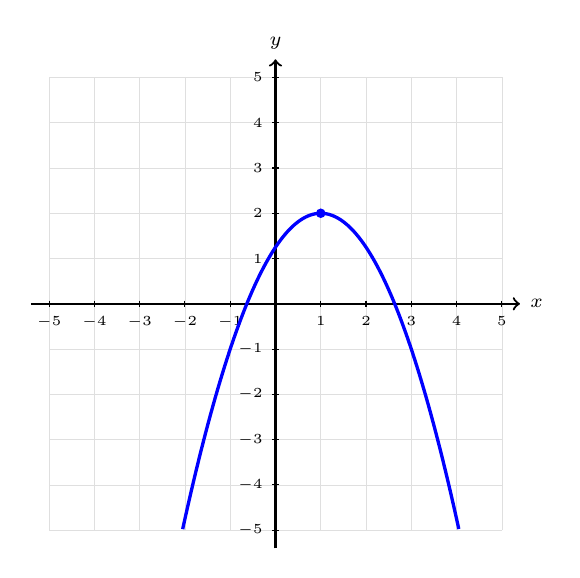
\begin{tikzpicture}[scale=0.575]
  \gridaxes{5}
  \draw[very thick,blue,domain=-2.05:4.05,samples=120] plot(\x,{-(3/4)*(\x-1)^2+2});
  \fill[blue] (1,2) circle (3pt);
\end{tikzpicture}
\par\vspace{9mm}\raggedright Equation: \underline{\hspace{4.5cm}}
\end{minipage}
% ===========================================================================
\newpage
\section*{Section 2 --- Completing the Square}
\subsection*{Reading --- turning $ax^2+bx+c$ into vertex form}
\textbf{Worked example ($a=1$).} Rewrite $x^2 + 6x + 1$ in vertex form.
\begin{align*}
  x^2 + 6x + 1
  &= \big(x^2 + 6x + (\tfrac{6}{2})^2\big) - 9 + 1 && \text{add and subtract } (b/2)^2 \\
  &= (x^2 + 6x + 9) - 8 \\
  &= (x+3)^2 - 8. && \text{fold the perfect square}
\end{align*}
The key idea here is: take half the middle coefficient, \textbf{square it}, and add-and-subtract it so you can fold a
perfect square without changing the value.

\medskip
\textbf{Worked example ($a\neq 1$).} For $2x^2 - 12x + 5$, first \textbf{factor $a$ out of the $x$-terms}:
\[
  2x^2 - 12x + 5 = 2\big(x^2 - 6x\big) + 5 = 2\big(x^2 - 6x + 9 - 9\big) + 5 = 2\big((x-3)^2 - 9\big) + 5 = 2(x-3)^2 - 13 .
\]
\subsection*{Problems 16--21 --- complete the square}
Write each in the form $a(x-h)^2 + k$. Show your steps in the space below each problem.

\bigskip
\textbf{16.}\quad $x^2 + 6x + 5$

\vspace{3.2cm}
\textbf{17.}\quad $x^2 - 4x + 1$

\vspace{3.2cm}
\newpage
\textbf{18.}\quad $x^2 + 3x + 1$

\vspace{4cm}
\textbf{19.}\quad $2x^2 - 12x + 7$

\vspace{4cm}
\textbf{20.}\quad $3x^2 + 12x + 5$

\vspace{4cm}
\textbf{21.}\quad $-x^2 + 4x + 1$

\vspace{4cm}
% ===========================================================================
\newpage
\section*{Section 3 --- Putting It All Together}
\subsection*{Reading --- you cannot ``eyeball'' a parabola from $ax^2+bx+c$}
Looking at a raw quadratic like $x^2 - 6x + 11$, you \emph{cannot} tell where its vertex is or whether it crosses
the $x$-axis --- your intuition has almost nothing to grab onto. Completing the square is what reveals the
picture. Once it is in vertex form you can read the vertex, the direction, and the intercepts directly.
\subsection*{Problems 22--25}
For each: \textbf{(i)} complete the square to get vertex form \textbf{(ii)} graph it.

\medskip
\foreach \eq/\lbl in {{x^2-6x+11}/22, {x^2+4x+1}/23, {-x^2+2x+3}/24, {2x^2-8x+5}/25}{%
  \textbf{\lbl.}\quad $\displaystyle y=\eq$\par
  \vspace{4.5cm}
  Vertex form: \underline{\hspace{4.5cm}}
  \begin{center}\blankgrid[0.6]{6}\end{center}
  \vspace{6mm}
  \ifnum\lbl<25\relax\newpage\fi
}
% ===========================================================================
\newpage
\section*{$\bigstar$ Challenge Problems}
\textbf{26.}\quad$\bigstar$\quad \textbf{The biggest pen.} A rancher has $40$ meters of fencing to make a
rectangular pen, using a straight wall as one side (so the wall side needs no fence). All $40$ meters go into the
other three sides (which you are deciding the length of them). Let $w$ be the length of each of the two sides that stick out from the wall.

\medskip
\textbf{(a)}\quad As defined, the two sides sticking out from the wall each have length $w$, and the remaining fence forms the
side parallel to the wall. Using the fact that the three fenced sides total $40$ meters, write the length of the
side parallel to the wall in terms of $w$. Then, using area $=$ length $\times$ width, write a function $A(w)$ for
the enclosed area. \textit{(Sketching the pen first will help.)}
\vspace{10cm}

\newpage
\textbf{(b)}\quad Expand $A(w)$ and complete the square (or use the vertex formula) to find the width $w$ that gives
the \textbf{maximum} area, and state that maximum area. Explain why the vertex answers this question.

\newpage
\textbf{27.}\quad$\bigstar$\quad \textbf{Where the quadratic formula comes from.} Complete the square on the general
quadratic to \emph{derive} the quadratic formula. Start from
\[
  ax^2 + bx + c = 0 \qquad (a \neq 0),
\]
and follow the same steps you used all homework: factor $a$ out of the first two terms, complete the square, then
solve for $x$. You should arrive at
\[
  x = \frac{-b \pm \sqrt{b^2 - 4ac}}{2a}.
\]
% ===========================================================================
\end{document}
